	L'équipe avait émis le besoin de mettre en place des tests de charge, JMeter étant installé et y étant formé j'ai pris en charge la réalisation de ces tests. Ces derniers consistent à mesurer le temps de réponse d'un système lorsque celui-ci est soumis à des conditions particulières afin de vérifier s'il est capable de soutenir le traffic attendu. Les conditions regroupent différents paramètres comme le temps de réponse, le volume du traffic, le nombre de requêtes effectuées en parallèle, la configuration du matériel ou encore la stabilité des serveurs. Afin de réaliser de tels tests, il faut dans un premier temps configurer l'environnement sur lequel ils seront exécutés. Dans notre cas, nous avions à notre disposition un environnement de pré-production (RGB) dont les caractéristiques étaient identiques à celles de la production, ce qui était approprié pour réaliser ce genre de tests. De plus, nous avions aussi l'environnement HOMO3 avec des capacités inférieures, idéal pour exécuter les tests dans des conditions un peu plus extrêmes dans le but mesurer la robustesse des APIs. \\
	
	Après cela, j'ai pris soin de définir différents scénarios de tests dont l'objectif étaient de simuler l'activité utilisateur afin de se rapprocher le plus possible des cas d'utilisation réels. Par exemple, un des scénario classique pourrait décrire la procédure suivie pour effectuer une transaction bancaire d'un compte vers un autre. Pour cela, l'utilisateur pourrait se connecter à l'application mobile puis initier sa transaction en choisissant des comptes débiteur et créditeur et il enfin il la signerait numériquement. De plus, celui-ci pourrait d'abord consulter ses comptes avant de prendre la décision de réaliser cette transaction. Les scénarios sont représentés par des diagrammes de cas d'utilisation comme celui présent sur la figure \ref{scenarioTest}, décrivant la réalisation d'une transaction. \\

	On peut ainsi remarquer rapidement les différents services (listés en annexe \ref{a2}) qui seront appelés lors de l'exécution de ce scénario :
	\begin{itemize}
		\item VKB pour générer le clavier virtuel permettant l'authentification et la signature de la transaction
		\item tokenInfo pour générer le token d'authentification
		\item newTransfer pour initier la transaction
		\item accountToDebit pour sélectionner le compte débiteur
		\item addressBook pour sélectionner le compte créditeur
		\item signByVKB pour signer la transaction
		\item clientList pour lister tous les comptes
		\item accountOverview pour consulter un compte particulier \\
	\end{itemize}
	
	Une fois les services identifiés, il ne restait plus qu'à construire le plan de test JMeter permettant de réaliser le scénario. Pour cela, j'ai réemployé la structure mise en place précédemment pour les tests fonctionnels. Cependant, j'ai supprimé l'ensemble des assertions puisque ces dernières peuvent influer sur les temps de réponse calculés par JMeter et n'ont pas d'intérêt dans un test de charge. Il ne restait donc qu'à modifier les scripts Beanshell déjà écrits pour les adapter à la situation. La principale différence réside dans la configuration du moteur d'utilisateur. En effet, sur les tests fonctionnels j'avais placé un tel moteur à la racine des plans afin qu'il englobe tous les composants. Ainsi, pour les tests de charges il suffisait de modifier les paramètres du moteur à savoir le nombre de thread, d'itération et le temps de montée en charge pour adapter les conditions d'exécution des scénarios sans avoir à modifier la structure des plans. \\
	
	Ces tests de charges ont par la suite été exécutés dans différentes conditions ce qui a permis de déceler certaines anomalies. Par exemple, après avoir essayé d'envoyer un grand nombre de requêtes par seconde, nous nous sommes aperçus que beaucoup d'entre elles échouaient. Après une analyse approfondie, il s'est avéré qu'une grande partie retournaient un "timed out"; Cela provenait d'un problème de configuration de la gateway Zuul au sein de la couche microservices.
	
	Nous allons utiliser le schéma figure \ref{testChargeProbleme} afin d'expliciter le problème rencontré. Bien que le raisonnement expliqué soit réel, les chiffres ne le sont pas et ne sont présents que pour illustrer ce qui n'empêche pas la compréhension. JMeter envoie 1000 requêtes à la seconde qui passeront dans un premier temps par l'API Gateway d'Axway qui les traite sans soucis. Celle-ci peut donc forwarder l'ensemble des requêtes à l'API microservices qui seront alors interceptées par la gateway Zuul. Elle était configurée pour gérer 100 threads par seconde avec un timeout de 1 seconde. Cela signifie qu'elle peut traiter 100 requêtes par seconde et qu'elle rejette les requêtes donc le temps de traitement est supérieur à 1 seconde en tuant le processus. Il fallait donc revoir cette configuration à la hausse afin de résoudre le problème rencontré. Cependant, augmenter la taille du pool de threads que la gateway est capable de traiter par seconde aura forcément un impact sur le temps de réponse moyen des requêtes. Ainsi, une petite étude a été menée afin de déterminer une taille optimale permettant de traiter un nombre satisfaisant de requêtes tout en conservant un temps de réponse moyen correct. Pour cela plusieurs tests de charge ont été effectués avec des configurations différentes et nous avons procédé par dichotomie pour trouver les valeurs les plus satisfaisantes (exemple tableau \ref{tableauThreads}). De plus, nous avons attendu confirmation d'EFS sur la capacité de ses API afin de ne pas risquer une congestion à la sortie de la couche microservices.
	
\begin{figure}[h!]
	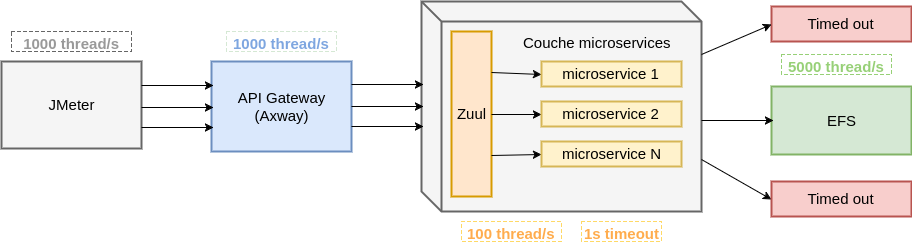
\includegraphics[scale=0.5]{images/travailNeuflizeOBC/testsFonc/testChargeProbleme.png}
	\centering
	\caption{Traitement des threads par les différentes couches}
	\label{testChargeProbleme}
\end{figure}

\begin{table}[h!]
	\center
	\begin{tabular}{| c | c |}
     \hline
     Threads/s & Temps de réponse moyen (ms)\\ \hline
     100 & 300 \\ \hline
     300 & 350 \\ \hline
     500 & 420 \\ \hline
     700 & 750 \\ \hline
     1000 & 1250 \\
     \hline
	\end{tabular}
	\caption{Temps de réponse moyen en fonction de la taille des pools de threads}
	\label{tableauThreads}
\end{table}